%\begin{enumerate}[label=\arabic*.,ref=\theenumi]
\begin{enumerate}[label=\thesection.\arabic*.,ref=\thesection.\theenumi]
\numberwithin{equation}{enumi}
%3.1
\item Discuss the relation between Stability and Phase Margin (PM).\\
\solution Let the loop gain
\begin{align}
L(s) = G(s)H(s)
\end{align}
Then the closed loop gain 
\begin{align}
T\brak{\j\omega} = \frac{G\brak{\j\omega}}{1+L\brak{\j\omega}}%\\
\end{align}
and 
%
If 
\begin{align}
\abs{L\brak{\j\omega_0}} &= 1,
\\
T\brak{\j\omega_0} &= \frac{G\brak{\j\omega_0}}{1+L\brak{\j\omega_0}}\\
\\
 &= \frac{G\brak{\j\omega_0}}{1+\exp\cbrak{\phase{L\brak{\j\omega_0}}}},
\end{align}
and 
\begin{align}
PM = 180^{\degree} - \phase{L\brak{\j\omega_0}}
\end{align}
%
and for
\begin{align}
PM
\begin{cases}
> 0 & T(s) \text{ stable}
\\
= 0 & T(s) \text{ marginally stable}
\\
< 0 & T(s) \text{ unstable}
\end{cases}
\end{align}
%------------------------------------------------------------------------------------------------------%
% 3.2
%\item If Phase of Loop Gain is $\phi$ at which the magnitude of loop gain is unity. Find range of $\phi$ for the system to be Stable, Marginally Stable and Unstable.\\
%\solution
%\begin{align}
%\phi = \alpha - 180^{\degree}\\
%\alpha = \phi + 180^{\degree}
%\end{align}
%
%For Stable,
%\begin{align}
%\alpha > 0\\
%\phi > -180^{\degree}
%\end{align}
%
%For Marginally Stable,
%\begin{align}
%\alpha = 0\\
%\phi = -180^{\degree}
%\end{align}
%
%For Unstable,
%\begin{align}
%\alpha < 0\\
%\phi < -180^{\degree}
%\end{align}
%------------------------------------------------------------------------------------------------------%
%3.3
\item For constant $H$, find the frequency at which $\phase{L\brak{\j\omega}} = -180^{\degree}$ and determine the region for Stability.
\solution

\begin{align}
\phase{G(f)H(f)} = \phase{G(f)}
\end{align}
\begin{multline}
\implies \phase{G(f)} = -180\degree
\\
=-\sbrak{\tan ^{-1}\brak{\frac{f}{10^{5}}}+\tan ^{-1}\brak{\frac{f}{10^{6}}}+\tan ^{-1}\brak{\frac{f}{10^{7}}}}
\end{multline}
or,
\begin{align}
f = f_{\pi} = 3.34 M Hz.
\end{align}

So, for 
\begin{itemize}
\item $f > 3.34 M Hz$, System is Unstable
\item $f = 3.34 M Hz$, System is Marginally Stable
\item $f < 3.34 M Hz$, System is Stable
\end{itemize}
%------------------------------------------------------------------------------------------------------%
%3.4
\item Determine the range of $H$ for Stability.\\
\solution
\begin{align}
\abs{G(f_{\pi})} &= 320 - 40\log(f_{\pi})\\
 &= 59 dB = 896\\
H &= 1.11 \times 10^{-3} \brak{\because \abs{G(f_{\pi})H} = 1}
\end{align}

%If $f$ \textbf{decreases} below $f = 3.34\times 10^6 Hz$, $G$ increases and the value of $H$ at which Loop-Gain becomes unity \textbf{decreases} below $H = 1.11 \times 10^{-3}$.

Thus, 
\begin{itemize}
\item $H > 1.11 \times 10^{-3}$, System is Unstable
\item $H = 1.11 \times 10^{-3}$, System is Marginally Stable
\item $H < 1.11 \times 10^{-3}$, System is Stable
\end{itemize}

\item Verify the stablity from the value of $H=9.9\times 10^{-3}$\\
\solution\\
\textbf{System is Unstable} as $H>1.11\times 10^{-3}$.

Run the following code to verify the stablity of the system
\begin{lstlisting}
codes/ee18btech11014/Stability.py
\end{lstlisting}

\item Using ngspice, find the Unit-Step Response for System for $H=9.9\times 10^{-3}$\\
\solution\\
 At $H=9.9\times 10^{-3}$, the Phase-Margin($\alpha$) of the system is
\begin{align}
\alpha \approx -38.5^{\circ}
\end{align}
So the system is \textbf{Unstable}.

Check the following spice file for circuit.
\begin{lstlisting}
spice/ee18btech11014/ee18btech11014_3.net
\end{lstlisting}

Following are the instructions to run the spice file.
\begin{lstlisting}
spice/ee18btech11014/README.md
\end{lstlisting}

Run the following code to see the Unit Step Response of Closed-Loop System for $H=9.9\times 10^{-3}$.
\begin{lstlisting}
spice/ee18btech11014/EE18BTECH11014_Simulation-3.py
\end{lstlisting}

The Unit-Step Response is Fig. \ref{fig:Unstable System}
\begin{figure}[ht!]
	\begin{center}
		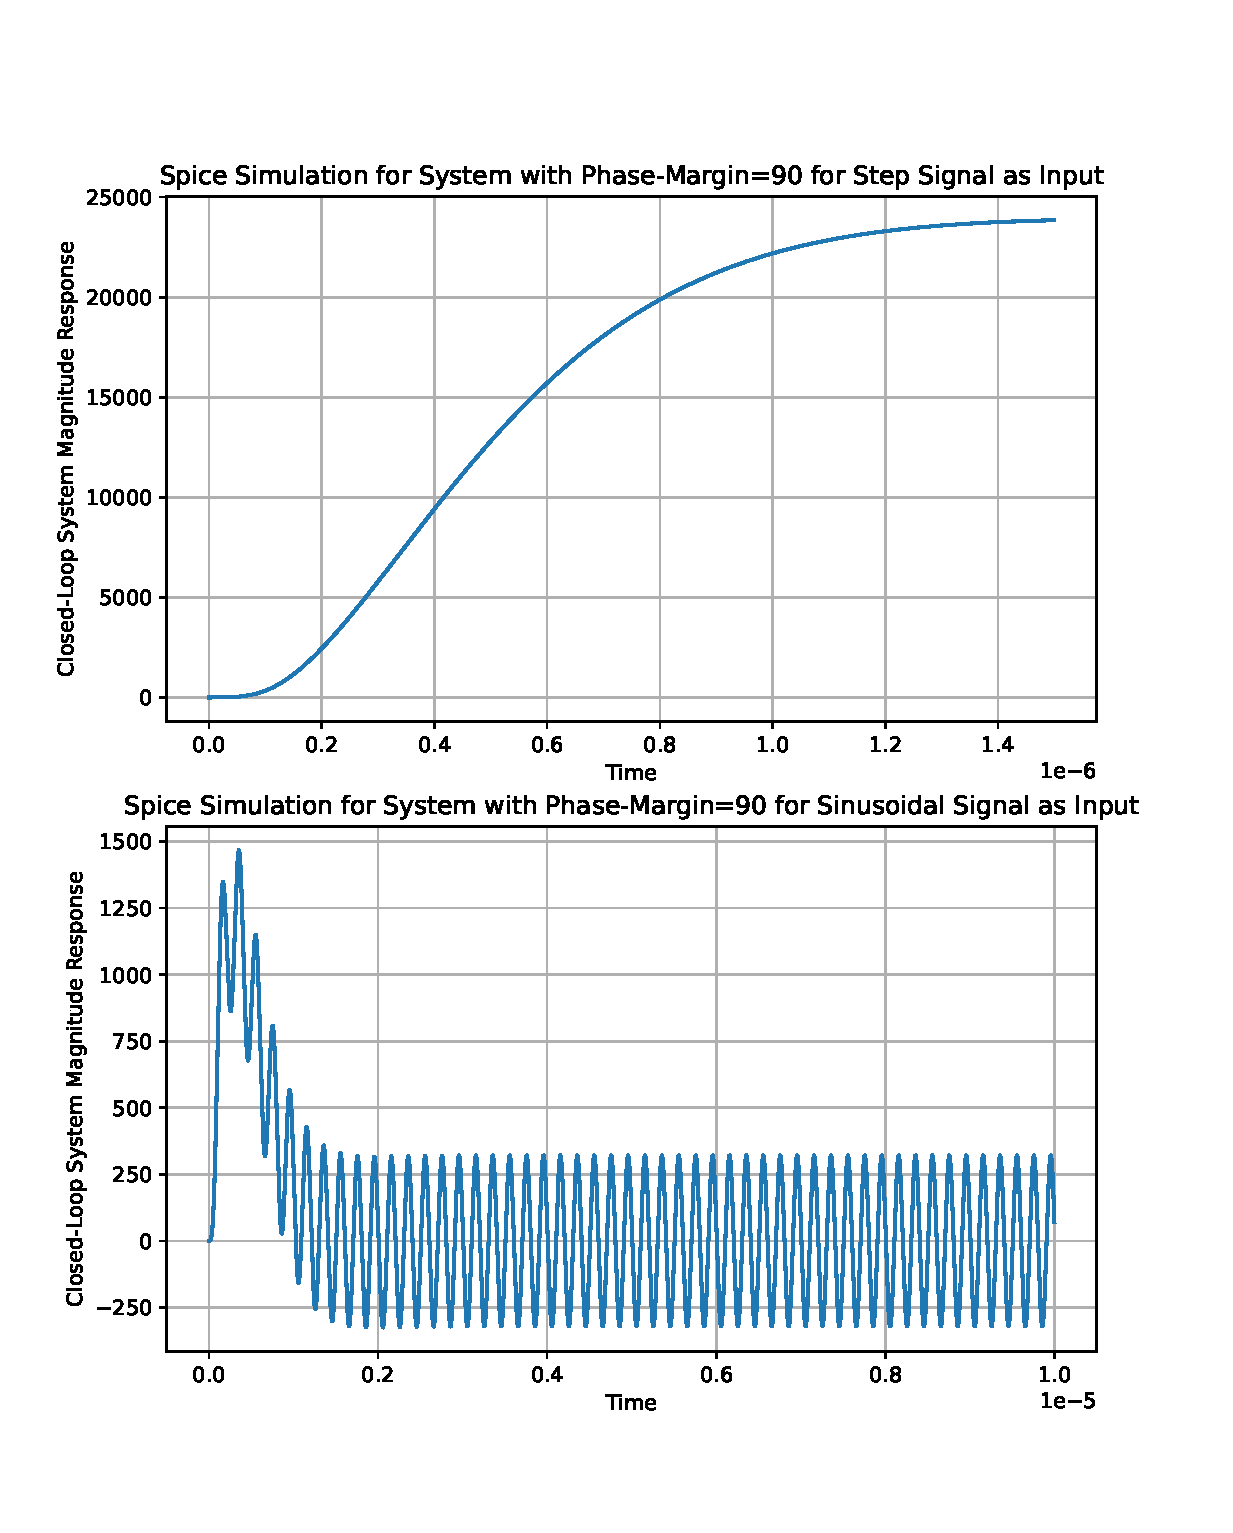
\includegraphics[width=\columnwidth]{./figs/ee18btech11014/ee18btech11014_Spice_Result.eps}
	\end{center}
	\caption{}
	\label{fig:Unstable System}
\end{figure}
\end{enumerate}
